\documentclass[12pt]{article}
%\documentclass[border=0.1cm]{standalone}
\usepackage{wasysym}
\usepackage{phonenumbers}
\usepackage{marvosym}
\usepackage{xcolor}
\usepackage[super]{nth}
\usepackage[paperwidth=8.5in,paperheight=11in,margin=0.45in]{geometry} 
\usepackage[USenglish]{babel}
\usepackage[USenglish]{isodate}% http://ctan.org/pkg/isodate
\usepackage[final]{pdfpages}
\usepackage{hyperref}
\hypersetup{
  colorlinks   = true, %Colours links instead of ugly boxes
  urlcolor     = black, %Colour for external hyperlinks
  linkcolor    = black, %Colour of internal links
  citecolor    = black %Colour of citations
}
\usepackage[activate={true,nocompatibility},final,tracking=true,kerning=true,spacing=true,factor=1100,stretch=10,shrink=10]{microtype}
\frenchspacing
\usepackage[nodayofweek,level]{datetime}
\usepackage{calc,url}
\newcounter{qz}\setcounter{qz}{0}
\newcommand{\qz}{%\
\setcounter{qz}{\value{qz}+1}
\textbf{In-class  \theqz} \,}

\newcounter{hw}\setcounter{hw}{0}
\newcommand{\hw}{%\
\setcounter{hw}{\value{hw}+1}
\textbf{HW \thehw}}

\newcounter{ex}\setcounter{ex}{0}
\newcommand{\ex}{%\
\setcounter{ex}{\value{ex}+1}
Exam \theex}

\usepackage[T1]{fontenc} 
\usepackage{fourier}
%\usepackage{tgschola} %to look retro
\newenvironment{mypar}[2]
  {\begin{list}{}%
    {\setlength\leftmargin{#1}
    \setlength\rightmargin{#2}}
    \item[]}
  {\end{list}}


\newcounter{wk}\setcounter{wk}{0}
\newcommand{\wk}{%\
\setcounter{wk}{\value{wk}+1}
\thewk \,\,}

\usepackage[nomessages]{fp}% http://ctan.org/pkg/fp


\usepackage{enumerate}
\usepackage{graphicx}

\usepackage{paralist}
\renewenvironment{description}[0]{\begin{compactdesc}}{\end{compactdesc}}

\newenvironment{alphalist}{
  \begin{enumerate}[(a)]
    \addtolength{\itemsep}{-0.75\itemsep}}
  {\end{enumerate}}
  \cleanlookdateon% Remove ordinal day reference
  \newcommand{\RomanNumeralCaps}[1]
      {\MakeUppercase{\romannumeral #1}}

\usepackage{xspace}
\makeatletter
\DeclareRobustCommand{\maybefakesc}[1]{%
  \ifnum\pdfstrcmp{\f@series}{\bfdefault}=\z@
    {\fontsize{\dimexpr0.8\dimexpr\f@size pt\relax}{0}\selectfont\uppercase{#1}}%
  \else
    \textsc{#1}%
  \fi
}
\newcommand\AM{\maybefakesc{am}\xspace}
\newcommand\PM{\maybefakesc{pm}\xspace}
\makeatother

 \newcommand{\coursename}{Foundations of Mathematics}
\newcommand{\coursenumber}{MATH 250}
\newcommand{\sectionnumber}{01}
\newcommand{\term}{Spring }
\newcommand{\room}{Discovery Hall, room 386}
\newcommand{\meetingtime}{This class meets Monday, Wednesday, and Friday in \room \/  from 2:30\PM to 3:20\PM.}
\newcommand{\officehours}{Monday, Wednesday, and Friday 10:00\AM-11:00\AM,
    Tuesday and Thursday 12:00 noon-2:00\PM, and by appointment.}

\begin{document}
\cleanlookdateon% Remove ordinal day reference
\shortdate
\printyearoff
\large
\begin{center}
    \textbf{\coursename}  \\
    {\coursenumber--\sectionnumber} \\
     {\term \the\year} \\
\end{center}

\vskip0.25in
\normalsize


\begin{center}
\begin{description}
    \item[Instructor:] Barton Willis, PhD, Professor of Mathematics
    \item[Office:]  Discovery Hall, Room 368
    \item[\phone:]   \phonenumber[country=US]{3088658868}
    \item[\Email:]    \href{mailto:willisb@unk.edu}{willisb@unk.edu}
    \item[Zoom for classes:] For Zoom class meetings, use the Meeting ID: 616 568 5706. 
    \item[Office Hours:] \officehours
  \end{description}
\end{center}

\subsubsection*{Class meeting time and place}

\meetingtime



\subsubsection*{Course Resources}

\noindent Our textbook is \emph{Introduction to Mathematical Structures and Proofs}, \nth{2} edition,  by  Larry Gerstein.
Some homework assignments for this course will need to be typeset. To do this, you will need to create a \emph{no cost} 
account on Overleaf (\url{https://www.overleaf.com/}).   For  tutorial for using Overleaf, see \url{https://www.overleaf.com/tutorial}.



\subsubsection*{Important Dates}

\begin{mypar}{0.25in}{0.25in} 

      \textbf{First Homework due} \dotfill  \textbf{\printdate{28/1/\the\year}}  \\
       \textbf{Exam 1} \dotfill \textbf{\printdate{17/2/\the\year}}  \\
    \textbf{Exam 2} \dotfill  \textbf{\printdate{24/3/\the\year}} \\
    \textbf{Exam 3} \dotfill \textbf{\printdate{21/4/\the\year}} \\
      \textbf{Final exam} \dotfill  \textbf{\printdate{15/5/\the\year}, 3:30 \PM  --  5:30 \PM}
\end{mypar}



\subsubsection*{Grading}

Your course grade will be based on weekly homework sets, three midterm exams, and a comprehensive 
final exam; specifically:
\begin{mypar}{0.25in}{0.25in}
    \textbf{Weekly Homework}  \emph{11 fifteen point assignments}  \dotfill 165 (total) \\
    \textbf{Mid-term exams 1,2, and 3} \emph{100 points each} \dotfill 300 (total)\\
      \textbf{Comprehensive Final exam} \dotfill 150 (total)
\end{mypar}
If it is necessary to adjust the number of  homework assignments,  your homework point 
total will be scaled to a total of 165.  For example, if we have only ten homework sets, 
your homework score will be scaled by a factor of \(165/150\).

\FPeval{\points}{round(165+300+150,0)}

\FPeval{\F}{round(\points*0.6-1,0)}
\FPeval{\Dm}{round(\points*0.6,0)}
\FPeval{\D}{round(\points*0.63,0)}
\FPeval{\Dp}{round(\points*0.66,0)}

\FPeval{\Cm}{round(\points*0.7,0)}
\FPeval{\C}{round(\points*0.73,0)}
\FPeval{\Cp}{round(\points*0.76,0)}

\FPeval{\Bm}{round(\points*0.8,0)}
\FPeval{\B}{round(\points*0.83,0)}
\FPeval{\Bp}{round(\points*0.86,0)}

\FPeval{\Am}{round(\points*0.9,0)}
\FPeval{\A}{round(\points*0.93,0)}
\FPeval{\Ap}{round(\points*0.98,0)}
The following table shows the \emph{minimum} number of points (out of \points) that
are required for each of the twelve letter grades D- through A+. For
example, a point total of \Bp\/  points will earn you a grade of B+,  and 
a point total of \Am\/ points will earn you a grade of A-. A point
total of \F\/  or less earns you a failing course grade.
 
 \vspace{0.1in}
     \begin{minipage}{5.5in}
  \centering 
\begin{mypar}{0.25in}{0.25in}
    \begin{minipage}{2.5in}
        D-  \dotfill \Dm \\
        D \dotfill \D \\
        D+ \dotfill \Dp \\
        C- \dotfill \Cm  \\
        C \dotfill \C \\
        C+ \dotfill \Cp 
        \end{minipage}
    \phantom{xxx}
    \begin{minipage}{2.5in}
        B- \dotfill \Bm \\
        B \dotfill  \B \\
        B+ \dotfill  \Bp\\
        A- \dotfill  \Am \\
        A \dotfill  \A \\
        A+ \dotfill  \Ap
    \end{minipage}
\end{mypar} 
\end{minipage}

\subsubsection*{Prerequisite}

The prerequisite for MATH 250 is an earned grade of D- or higher in either MATH 115 or MATH 123.

\subsubsection*{Catalog description}

\textbf{Foundations of Mathematics (3 credit hours)} Topics of sets and symbolic logic are studied with the objective of using them in the detailed study of the nature of different types of proofs used in mathematics. Also, the processes of problem solving are studied for developing strategies of problem solving.

\subsubsection*{Learning Outcomes}

On completion of this course, students will
\begin{alphalist}
    \item gain an understanding of na\"ive set theory. 
    \item gain an understanding of symbolic logic, quantifiers, and functions.
    \item gain an understanding of direct proofs, proofs by contradiction, proofs by contrapositive, and proofs by induction.
    \item gain the ability to read and understand mathematical proofs.
    \item gain the problem solving skills that are needed to create a mathematical proof.
\end{alphalist}

\subsubsection*{Course Calendar}

Generally, we'll adhere to the scheduled exam dates even if we are ahead or behind with course work.  
When we are ahead or behind, the topics on the exams will be appropriately adjusted.  


\vspace{0.1in}
\noindent \textbf{Notices:}


\begin{alphalist}
   \item \emph{Exams will be given on the \textbf{Friday} of the week they are assigned.}
   

    \item Homework (\textbf{HW}) will be due at midnight on  Saturday of the week they are assigned.  


\end{alphalist}

\vspace{0.1in}

\begin{center}
    \small
\begin{tabular}  {|l|l|l|l|l|}
\hline
{\bf Week}  & \textbf{Week Starting} &  {\bf Section(s)} & {\bf Topic(s)} & \textbf{Assessment} \\
\hline \hline 
\wk    &  \printdate{23/1/\the\year} &    \S 1.1, \S 1.2  &  Logical connectives; Truth tables  & \hw  \\
\wk    & \printdate{30/1/\the\year}   &  \S1.3 &  Introduction to Overleaf; Conditional statements & \hw  \\
\wk    & \printdate{6/2/\the\year}&     \S1.4, \S1.5  &   Proof structures;  Logical equivalence &  \hw \\
\wk    & \printdate{13/2/\the\year}   &     \S2.1, \S2.2  & Sets; Russell's paradox   &   \textbf{\ex}       \\ \hline
\wk    & \printdate{20/2/\the\year} &  \S2.3, \S2.4    &  Quantifiers; Set inclusion   & \hw \\ 
\wk    & \printdate{27/2/\the\year}    & \S2.5, \S2.6   &  Union, intersection, complements; Indexed sets &    \hw  \\
\wk    & \printdate{6/3/\the\year}     & \S2.7, \S2.8  &  Power sets; Ordered pairs & \hw \\
\wk    & \printdate{20/3/\the\year}   & \S2.9  &  Set decompositions     &   \textbf{\ex}   \\ \hline
\wk   &  \printdate{27/3/\the\year}   & \S2.10 &  Induction   & \hw \\ 
\wk   &  \printdate{3/4/\the\year}      &   \S3.1 &  Functions &   \hw \\
\wk   &  \printdate{10/4/\the\year}   &   \S3.2, \S3.3 & One-to-one and onto functions; Function composition   & \hw  \\
\wk   & \printdate{17/4/\the\year}  & \S4.1, \S4.2  &  Cardinality; Finite and infinite sets   &   \textbf{\ex}  \\ \hline
\wk   & \printdate{24/4/\the\year} & \S4.3  &   Countable  and uncountable sets & \hw \\
\wk   & \printdate{1/5/\the\year}    &  \S5.1, \S5.2      & Combinatorial problems; Addition and product rules  &  \hw   \\
\wk   & \printdate{8/5/\the\year}   &  \S5.3, \S5.4      & Permutations; Geometric symmetry  &      \\
 \wk   & \printdate{15/5/\the\year}     &  &    \hfill  & \textbf{ Final Exam}  \\  \hline
   
\end{tabular}
\end{center}



\subsubsection* {Policies}

Unless an assessment is \emph{explicitly} stated to be a group project,  \emph{all work you turn in for a grade must be your own.}  If you need assistance in completing a homework assignment, you may ask me for help. Googling for answers, seeking help from the Learning Commons or other faculty members,  or using solution keys from previous terms (either from UNK or other universities) is also prohibited.  Violation of these rules will result in earning a grade of zero on the assessment. Each homework assignment you turn in for a grade must include the statement:

\begin{quote}
\fbox{I have neither given nor received unauthorized assistance on this assignment.}
\end{quote}
 If two assignments are so similar that only collaboration could explain their similarities, both assignments will receive a grade of zero.  Using unauthorized materials or communication devices (cell phone, for
example) while taking a test will earn you a grade of zero on that assessment.  
For the university academic integrity policy, please read
\small \url{https://catalog.unk.edu/undergraduate/academics/academic-regulations/academic-integrity-policy/}
 
\normalsize
Specially, our course policies are:
\begin{enumerate}

\item Regular in person class attendance is required. If you are ill or need to miss 
class due to athletics, please let me know ahead of time and I will make an effort to put the class on Zoom. 
Our classroom technology often doesn't work, so do not rely on watching recorded classes.

\item There is no explicit grade penalty for not attending class. But if you choose to not attend class for reasons other
than illness or athletics, I reserve the right to not be all that helpful in giving you assistance on homework or helping 
you learn missed material.

\item All examinations, including the final exam, must be taken in person.

\item For examinations and in class assignments, show your work.  \emph{No credit will be given for multistep problems without the necessary work. Your solution must contain enough detail
so that I am convinced that you could correctly work any similar problem.} Also erase or clearly mark any work you want me to ignore; otherwise,
I'll grade it.  

\item The work you turn in is expected to be \emph{accurate, 
complete, concise, neat}, and \emph{well-organized}.  
\emph{You will not earn full credit on work that falls short of 
these expectations.}

\item Class cancellations due to weather, illness, or other 
unplanned circumstances may require that we make  adjustments
to the course calendar, exam dates, due dates, or specifics for 
course assessments. 


\item Extra credit is not allowed. 



\item For examinations, you may use a teacher provided quick reference sheet, 
but no other reference materials. You may also use a pencil, eraser, 
and a scientific calculator. For examinations, your phone and all such
devices must be turned off and \emph{out of sight}. 

\item Generally, if you are ill or absent for any reason (including 
athletics), you must turn in your in class work on time. Permission to
turn in work late must be made before the due date, otherwise late in class work 
will count zero points.


 

\item During class time, please refrain from using electronic devices. If your 
device usage distracts your classmates, I will ask you to put it away. If it's my 
impression that you are often not paying attention in class, I reserve the right to 
decline to help you during office hours.

\item The final examination will be \emph{comprehensive} and it will be given 
during the  time scheduled by the University. Except for \emph{extraordinary circumstances}
you must take the exam at this time.
 
\item If you have questions about how your work has been graded, make an appointment with me immediately.


\item Please regularly check Canvas  to verify that your scores have 
been recorded correctly.  If I made a mistake in recording one of
your grades, I'll correct it provided you saved your paper.

\end{enumerate}

\newpage

\subsubsection*{Reporting Student Sexual Harassment, Sexual Violence or Sexual Assault}

Reporting allegations of rape, domestic violence, dating violence, sexual assault, sexual harassment, and stalking enables the University to promptly provide support to the impacted student(s), and to take appropriate action to prevent a recurrence of such sexual misconduct and protect the campus community. Confidentiality will be respected to the greatest degree possible. Any student who believes they may be the victim of sexual misconduct is encouraged to report to one or more of the following resources:
\begin{description}
    \item[Local Domestic Violence, Sexual Assault Advocacy Agency]\phonenumber[country=US]{3082372599}

    \item[Campus Police (or Security)]\phonenumber[country=US]{3088658911}
    
    \item[Title IX Coordinator]\phonenumber[country=US]{3088658655}

\end{description}
Retaliation against the student making the report, whether by students or University employees, will not be tolerated.

\subsubsection*{Students with Disabilities}

It is the policy of the University of Nebraska at Kearney to provide flexible and individualized reasonable accommodation to students with documented disabilities. To receive accommodation services for a disability, students must be registered with the UNK Disabilities Services for Students (DSS) office, 175 Memorial Student 
Affairs Building,  \phonenumber[country=US]{3088658214} or by 
email \href{mailto:unkdso@unk.edu}{unkdso@unk.edu}

\subsubsection*{Students Who are Pregnant}

It is the policy of the University of Nebraska at Kearney to provide flexible 
and individualized reasonable accommodation to students who are pregnant. 
To receive accommodation services due to pregnancy, students must contact 
the Student Health office at \phonenumber[country=US]{3088658218}. The following 
links provide information for students and faculty regarding pregnancy 
rights:
\small
\begin{enumerate}
  \item \url{https://thepregnantscholar.org/title-ix-basics/}
  \item \url{https://nwlc.org/resource/faq-pregnant-and-parenting-college-
  graduate-students-rights/UNK Statement of Diversity & Inclusion}
\end{enumerate}
\normalsize

\subsubsection*{UNK Statement of Diversity \& Inclusion}

UNK stands in solidarity and unity with our students of color, our Latinx and international students, our LGBTQIA+ students 
and students from other marginalized groups in opposition to racism 
and prejudice in any form, wherever it may exist. It is the job of 
institutions of higher education, indeed their duty, to provide a 
haven for the safe and meaningful exchange of ideas and to support 
peaceful disagreement and discussion. In our classes, we strive to 
maintain a positive learning environment based upon open 
communication and mutual respect. UNK does not discriminate on the 
basis of race, color, national origin, age, religion, sex, gender, 
sexual orientation, disability or political affiliation. 
Respect for the diversity of our backgrounds and varied life 
experiences is essential to learning from our similarities as well 
as our differences. The following link provides resources and other 
information regarding D\&I: \url{https://www.unk.edu/about/equity-access-diversity.php}

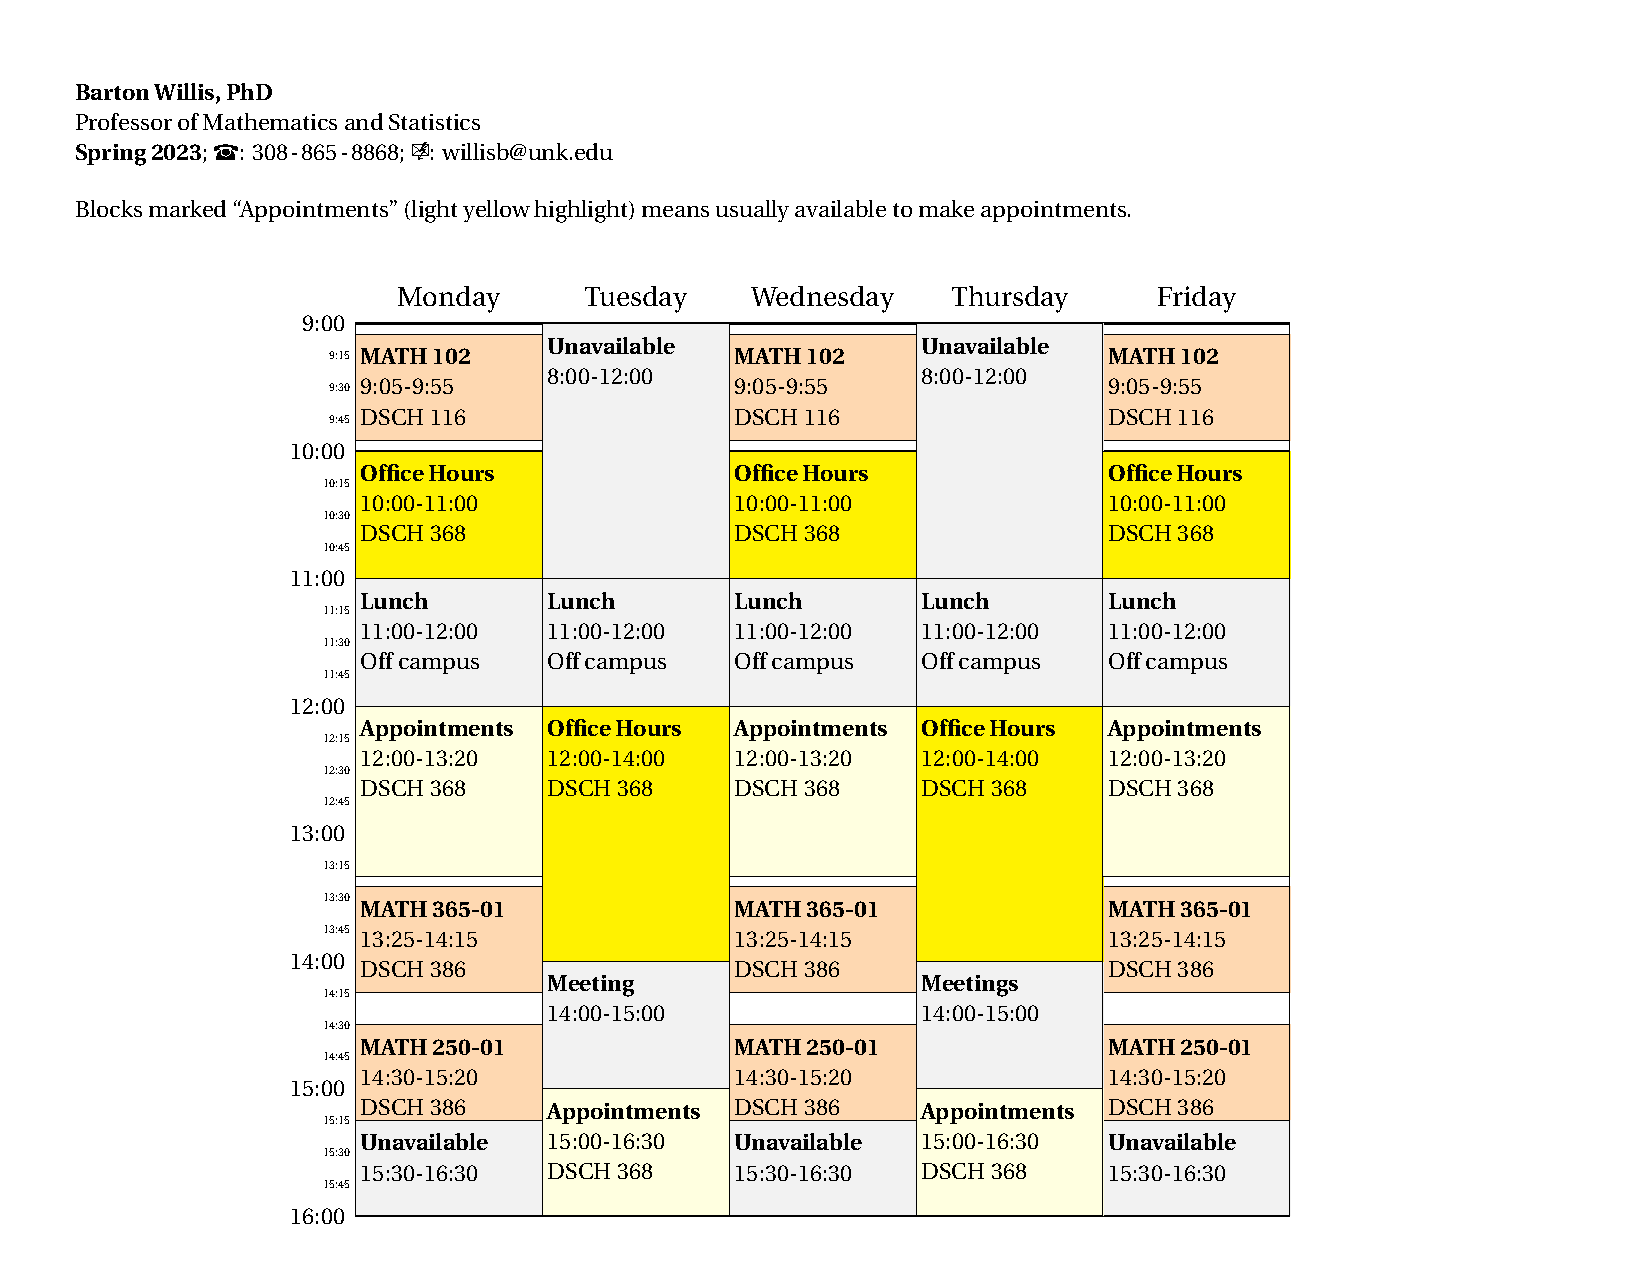
\includepdf[pages={1-},angle=90]{door-schedule.pdf}
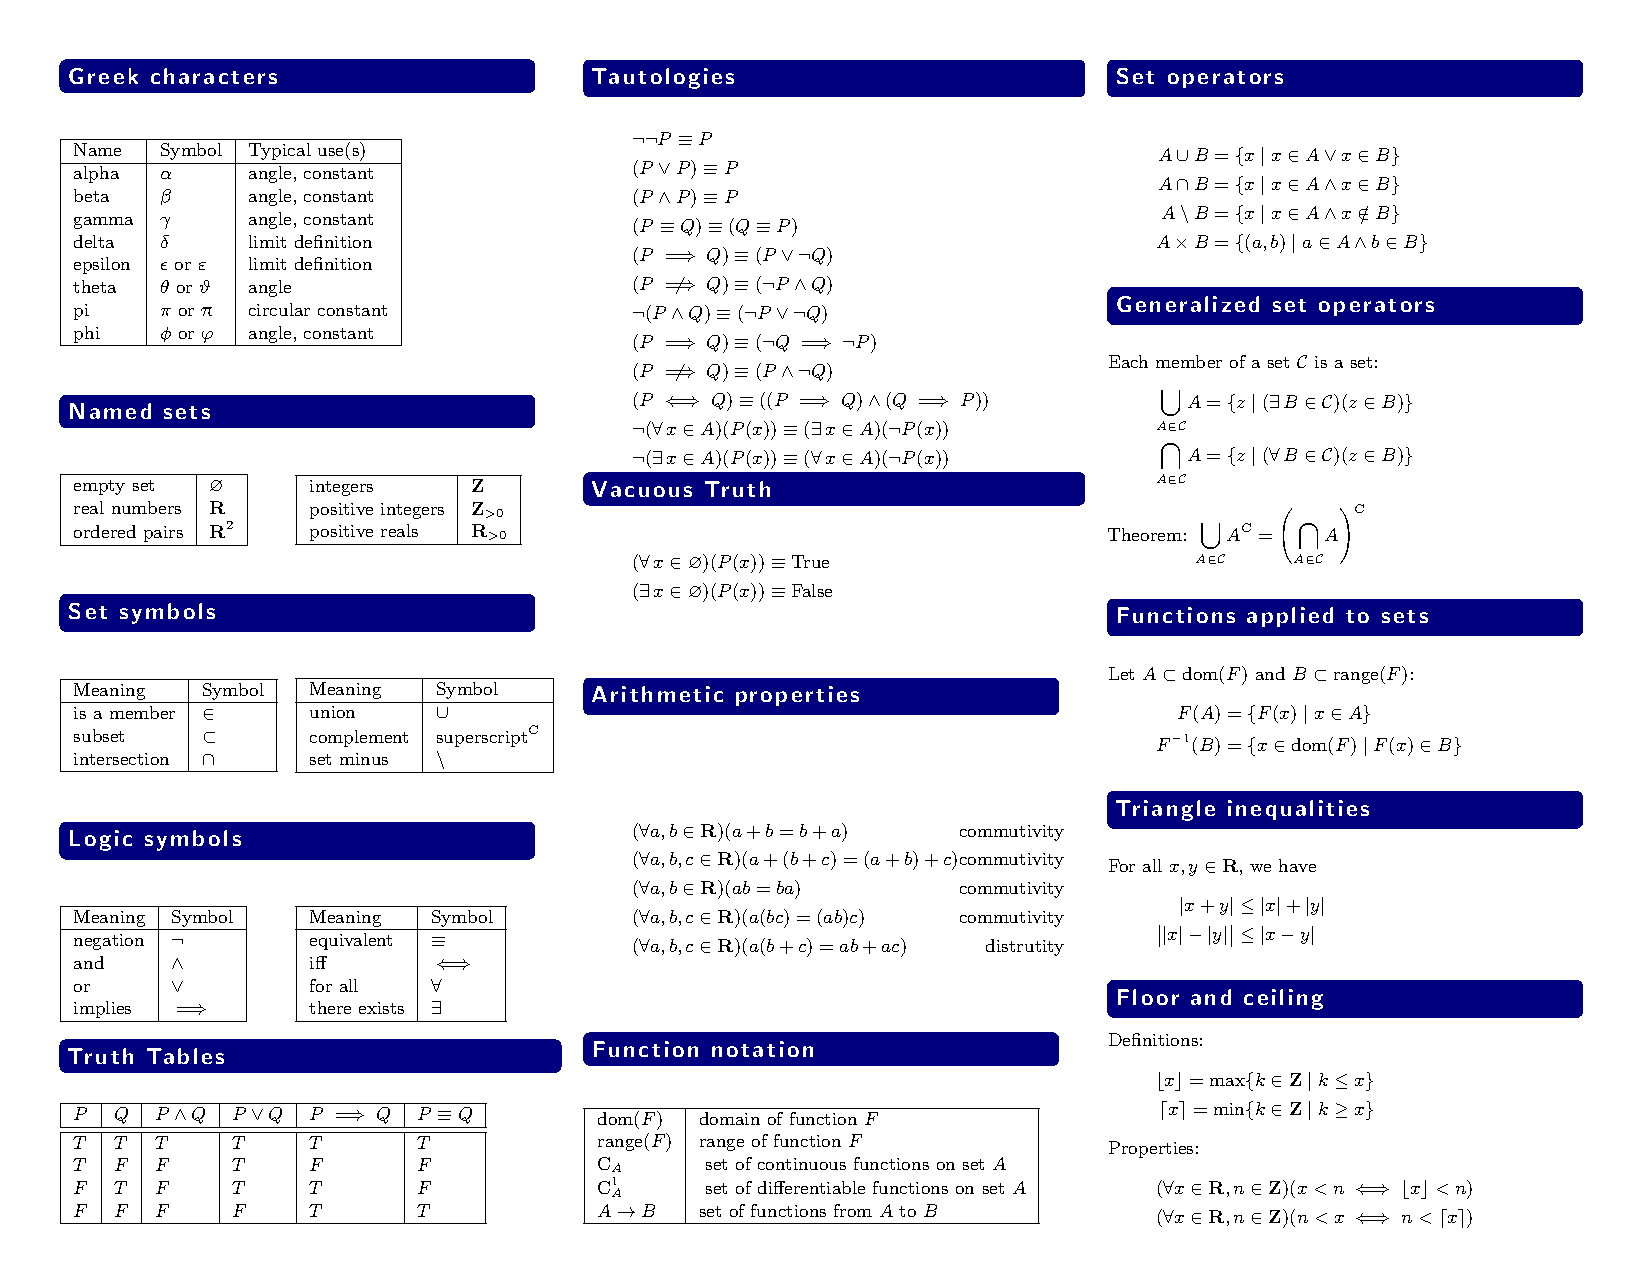
\includepdf[pages={1-},angle=90]{foundations-of-math-quick-reference.pdf}

\end{document}

